\documentclass[
  bibliography=totoc,     % Literatur im Inhaltsverzeichnis
  captions=tableheading,  % Tabellenüberschriften
  titlepage=firstiscover, % Titelseite ist Deckblatt
]{scrartcl}

% Paket float verbessern
\usepackage{scrhack}

% Warnung, falls nochmal kompiliert werden muss
\usepackage[aux]{rerunfilecheck}

% unverzichtbare Mathe-Befehle
\usepackage{amsmath}
% viele Mathe-Symbole
\usepackage{amssymb}
% Erweiterungen für amsmath
\usepackage{mathtools}

% Fonteinstellungen
\usepackage{fontspec}
% Latin Modern Fonts werden automatisch geladen
% Alternativ:
%\setromanfont{Libertinus Serif}
%\setsansfont{Libertinus Sans}
%\setmonofont{Libertinus Mono}
\recalctypearea % Wenn man andere Schriftarten gesetzt hat,
% sollte man das Seiten-Layout neu berechnen lassen

% deutsche Spracheinstellungen
\usepackage{polyglossia}
\setmainlanguage{german}


\usepackage[
  math-style=ISO,    % ┐
  bold-style=ISO,    % │
  sans-style=italic, % │ ISO-Standard folgen
  nabla=upright,     % │
  partial=upright,   % ┘
  warnings-off={           % ┐
    mathtools-colon,       % │ unnötige Warnungen ausschalten
    mathtools-overbracket, % │
},                       % ┘
]{unicode-math}

% traditionelle Fonts für Mathematik
\setmathfont{Latin Modern Math}
% Alternativ:
%\setmathfont{Libertinus Math}

\setmathfont{XITS Math}[range={scr, bfscr}]
\setmathfont{XITS Math}[range={cal, bfcal}, StylisticSet=1]

% Zahlen und Einheiten
\usepackage[
locale=DE,                   % deutsche Einstellungen
separate-uncertainty=true,   % immer Fehler mit \pm
per-mode=symbol-or-fraction, % / in inline math, fraction in display math
]{siunitx}

% chemische Formeln
\usepackage[
version=4,
math-greek=default, % ┐ mit unicode-math zusammenarbeiten
text-greek=default, % ┘
]{mhchem}

% richtige Anführungszeichen
\usepackage[autostyle]{csquotes}

% schöne Brüche im Text
\usepackage{xfrac}

% Standardplatzierung für Floats einstellen
\usepackage{float}
\floatplacement{figure}{htbp}
\floatplacement{table}{htbp}

% Floats innerhalb einer Section halten
\usepackage[
section, % Floats innerhalb der Section halten
below,   % unterhalb der Section aber auf der selben Seite ist ok
]{placeins}

% Seite drehen für breite Tabellen: landscape Umgebung
\usepackage{pdflscape}

% Captions schöner machen.
\usepackage[
  labelfont=bf,        % Tabelle x: Abbildung y: ist jetzt fett
  font=small,          % Schrift etwas kleiner als Dokument
  width=0.9\textwidth, % maximale Breite einer Caption schmaler
]{caption}
% subfigure, subtable, subref
\usepackage{subcaption}

% Grafiken können eingebunden werden
\usepackage{graphicx}
% größere Variation von Dateinamen möglich
\usepackage{grffile}

% schöne Tabellen
\usepackage{booktabs}

% Verbesserungen am Schriftbild
\usepackage{microtype}

% Literaturverzeichnis
\usepackage[style=alphabetic,]{biblatex}
% Quellendatenbank
\addbibresource{lit.bib}
\addbibresource{programme.bib}

% Hyperlinks im Dokument
\usepackage[
  unicode,        % Unicode in PDF-Attributen erlauben
  pdfusetitle,    % Titel, Autoren und Datum als PDF-Attribute
  pdfcreator={},  % ┐ PDF-Attribute säubern
  pdfproducer={}, % ┘
]{hyperref}
% erweiterte Bookmarks im PDF
\usepackage{bookmark}

% Trennung von Wörtern mit Strichen
\usepackage[shortcuts]{extdash}

\title{V51: Der Operationsverstärker}
\author{
  Simon Schulte
  \texorpdfstring{
    \\
    \href{mailto:simon.schulte@udo.edu}{simon.schulte@udo.edu}
  }{}
  \texorpdfstring{\and}{, }
  Tim Sedlaczek
  \texorpdfstring{
    \\
    \href{mailto:tim.sedlaczek@udo.edu}{tim.sedlaczek@udo.edu}
  }{}
}
\publishers{TU Dortmund – Fakultät Physik}

\date{Durchführung: 11.07.2018\\
      Abgabe: 14.09.2018}


\begin{document}

\maketitle
\thispagestyle{empty}
\setcounter{page}{1}
\pagenumbering{arabic}
\section{Theorie}
\label{sec:theorie}
In diesem Versuch werden verschiedene
Schaltungen mit Hilfe des Operationsverstärkers realisiert.
Zunächst wird auf die physikalischen Eigenschaften eingegangen,
woraufhin verschiedene Schaltungen skizziert und schließlich
realisiert werden.

\subsection{Eigenschaften des Operationsverstärkers}
\label{subsec:eigenschaften}
Die wichtigste elektrische Eigenschaft des Operationsverstärkers, auch
Differenzverstärker ist die Proportionalität der Ausgangsspannung $U_\text{A}$ zur
Differenz der Eingangsspannungen $U_\text{P}$ und $U_\text{N}$:
\begin{equation}
\label{eq:proportionalität}
    U_\text{A} = V(U_\text{P} - U_\text{N})\,,
\end{equation}
wobei $V$ die Leerlaufverstärkung bezeichnet.
Diese Beziehung gilt in einem Spannungsbereich
$-U_\text{B} < U_\text{A} < U_\text{B}$, der durch die Betriebsspannung
$U_\text{B}$ bestimmt ist. Außerhalb dieses Bereichs läuft die
Ausgangsspannung in eine Sättigung.

\noindent
Aus dem Zusammenhang für $U_\text{A}$ ergibt sich, dass für eine positive Spannung
bei $U_\text{N}$ und $U_\text{P} \less U_\text{N}$ die Ausgangsspannung negativ wird.
Daher nennt man den negativen Eingang auch den invertierenden Eingang und den positiven
Eingang auch den nicht invertierenden.
Die Grundschaltung eines Operationsverstärkers ist in Abbildung \ref{fig:op} dargestellt.
\begin{figure}
    \centering
    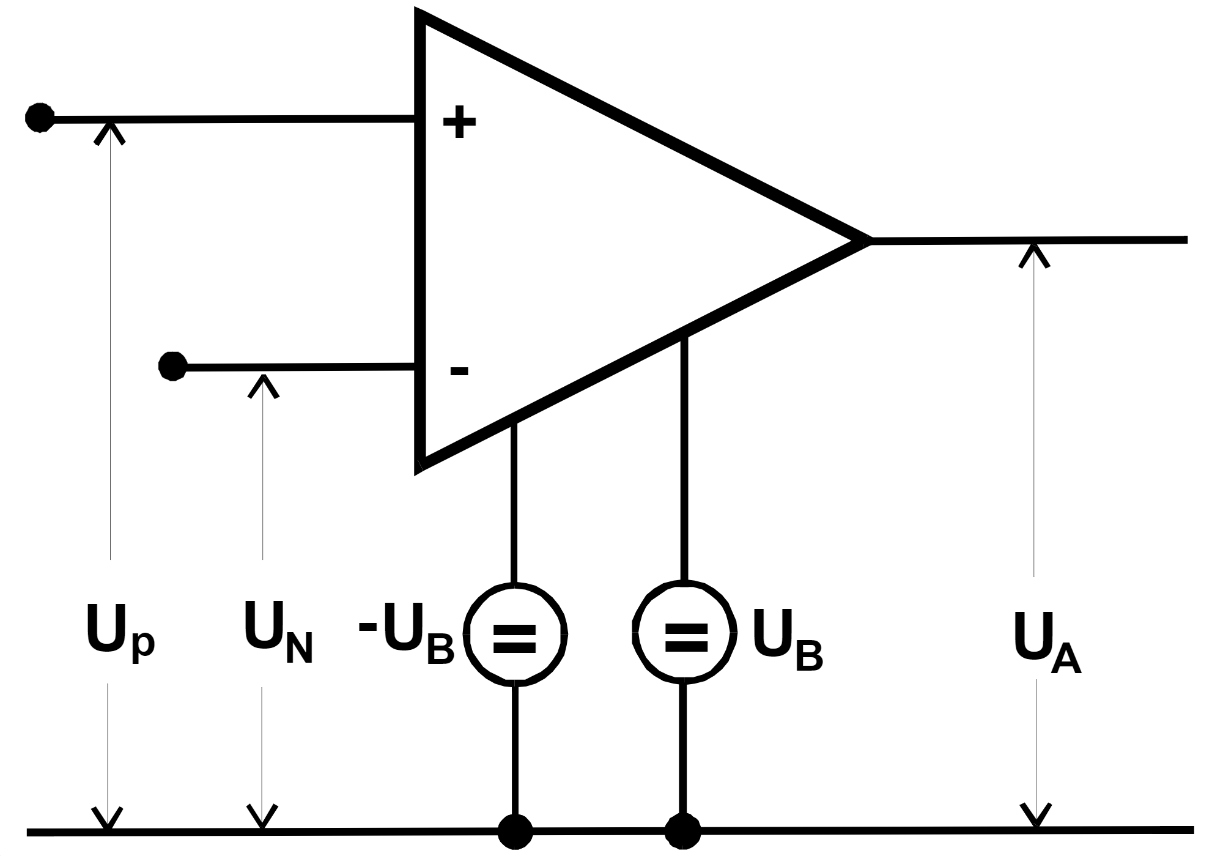
\includegraphics[width=0.5\linewidth]{op.PNG}
    \caption{
        Schaltbild eines Operationsverstärkers mit Ausgangsspannung
        $U_\text{A}$ und Eingangsspannungen $U_\text{P}$ und
        $U_\text{N}$ \cite{V51}.
    }
    \label{fig:op}
\end{figure}

\noindent
Neben der meist frequenzabhängigen Leerlaufverstärkung $V$ besitzt der
Operationsverstärker weitere Kenngrößen, wie die Eingangswiderstände,
$r_\text{e,P}$ und $r_\text{e,N}$, sowie
einen Ausgangswiderstand $r_\text{a}$.
Um Rechnungen zu Vereinfachen gilt für einen idealen Operationsverstärker
\begin{equation}
\label{eq:id-verstärker}
    V = \infty\,,\qquad r_\text{e} = \infty\,,\qquad r_\text{a} = 0\,.
\end{equation}
Aufgrund dieser Annahmen eines idealen Operationsverstärkers lassen sich die
Schaltungen mit einem Operationsverstärker relativ einfach nach Knoten- und Maschenregel
berechnen. Dabei spielt nur die äußere Beschaltung des OPVs eine Rolle.\\

\noindent
Im Gegensatz dazu müssen zur theoretischen Beschreibung eines realen
Operationsverstärkers zusätzliche Kenngrößen in Betracht gezogen werden.
\noindent
Die Gleichtaktverstärkung
\begin{equation}
\label{eq:gleichtaktverstärkung}
    V_\text{Gl} = \frac{\Delta U_\text{A}}{\Delta U_\text{Gl}}
\end{equation}
berücksichtigt geringe Asymmetrien der beiden Vertärkungskanäle.
Dabei bezeichnen $\Delta U_\text{A}$ die Differenz der Ausgangsspannung zu
\num{0} und $\Delta U_\text{Gl}$ den Unterschied der eigentlich gleichen
Eingangsspannungen.
\noindent
Die auf Grund endlicher Eingangswiderstände $r_\text{e}$ auftretenden
Eingangsströme werden mit $I_\text{P}$ und $I_\text{N}$, deren
Mittelwert,
\begin{equation}
\label{eq:eingangsruhestrom}
    I_\text{B} = \frac{1}{2}\left(I_\text{P} + I_\text{N}\right)\,,
\end{equation}
als Eingangsruhestrom und die Differenz
\begin{equation}
\label{eq:offsetstrom}
    I_0 = I_\text{P} - I_\text{N}\,,
\end{equation}
als Offsetstrom bezeichnet.
Ähnlich zum Offsetstrom, verschwindet auch die Spannung häufig nicht.
Für die Offsetspannung $U_0$ gilt daher bei $U_\text{A} = 0$
\begin{equation}
\label{eq:offsetspannung}
    U_0 = U_\text{P} - U_\text{N}\,.
\end{equation}
Sie ist abhängig von Temperatur, Zeit und Betriebsspannungen. Die totale
Ableitung wird mit Offsetspannungsdrift bezeichnet.


\section{Schaltungsbeispiele}
\label{sec:schaltungsbeispiele}
Im Folgenden werden einige Schaltbeispiele für Operationsverstärker
dargestellt.

\subsection{Rückgekoppelter Linearverstärker}
\label{subsubsec:rueck-linearverstärker}
Der relativ kleine Arbeitsbereich des Operationsverstärkers ist in der
Anwendung oft nicht praktikabel. Um diesen Bereich zu verbreitern, wird die
Verstärkung reduziert, indem ein Teil der Ausgangsspannung auf den
invertierenden Eingang gegeben wird. (Gegenkopplung).
Der Anteil der zurückgeführten Spannung kann dabei mit Hilfe der Widerstände
$R_1$ und $R_\text{N}$ bestimmt werden, die in Abbildung \ref{fig:linear}
dargestellt sind.
\begin{figure}[H]
    \centering
    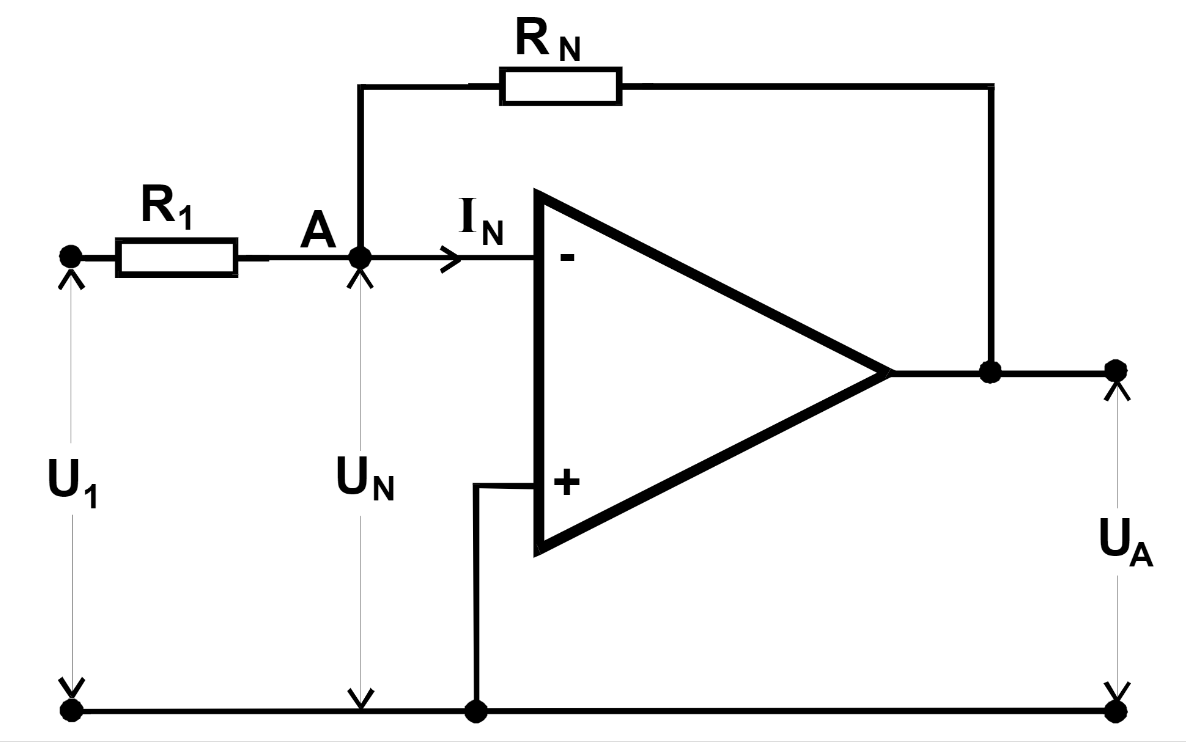
\includegraphics[width=0.5\linewidth]{linearverstaerker.PNG}
    \caption{Gegengekoppelter Linearverstärker \cite{V51}.}
    \label{fig:linear}
\end{figure}
\noindent
$U_N$ ist aufgrund der hohen Leerlaufverstärkung $V$ nahezu Null. Bei Betrachtung
des idealen Operationsverstärkers wird $U_N$ sogar exakt Null, da dort
$V -> \inf$. Beim idealen Operationsverstärker verschwindet außerdem
der Eingangsstrom IN. Daraus folgt mit der Kirchhoffschen Knotenregel für
den Verzweigungspunkt A:
\begin{equation}
  \frac{U_1}{R_1} + \frac{U_A}{R_N}\,=\,0.
\end{equation}
Die Verstärkung $V^\prime$ ist das Verhältnis von Ausgangsspannung $U_A$ zur Eingangsspannung
$U_1$. Daraus ergibt sich
\begin{equation}
  V^\prime = -\frac{R_\text{N}}{R_1}.
  \label{eqn:v'lingegen}
\end{equation}
Für den Fall $R_\text{N}/R_1 \ll V$ gilt dies auch für den realen OPV.
Der Geringe Eingangswiderstand $r_\text{e} \approx R_1$ wirkt sich bei
hochohmigen Spannungsquellen möglicherweise nachteilig auf Spannungsmessungen aus.
Im nächsten Abschnitt wird daher ein Linearverstärker vorgestellt, der diesen Nachteil
umgeht.




\subsection{Umkehr-Integrator und -Differentiator}
\label{subsec:integrator}
Mit Hilfe eines zusätzlichen Kondensators mit Kapazität $C$ in der Schaltung
eines Linearverstärkers lässt sich entweder ein Integrations- oder eine
Differentiationsglied bauen.
Für die Ausgangsspannungen $U_\text{A,I}$ des Integrators und $U_\text{A,D}$
des Differentiators gilt dann
\begin{align*}
    U_\text{A,I} &= - \frac{1}{RC} \int U_1\!(t) \mathup{d}t\,,\\
    \text{und} \qquad U_\text{A,D} &= - RC \frac{\mathup{d}U_1}{\mathup{d}t}\,.
\end{align*}
Dabei bezeichnet $R$ den Widerstand.
Integrator und Differentiator besitzen also Tief- und Hochpass Eigenschaften und
unterscheiden sich nur durch die Positionen des Widerstandes und des Kondensators.
Die entsprechenden Schaltungen sind in Abbildung \ref{fig:integrator} dargestellt.
\begin{figure}[H]
    \begin{subfigure}{.49\linewidth}
        \centering
        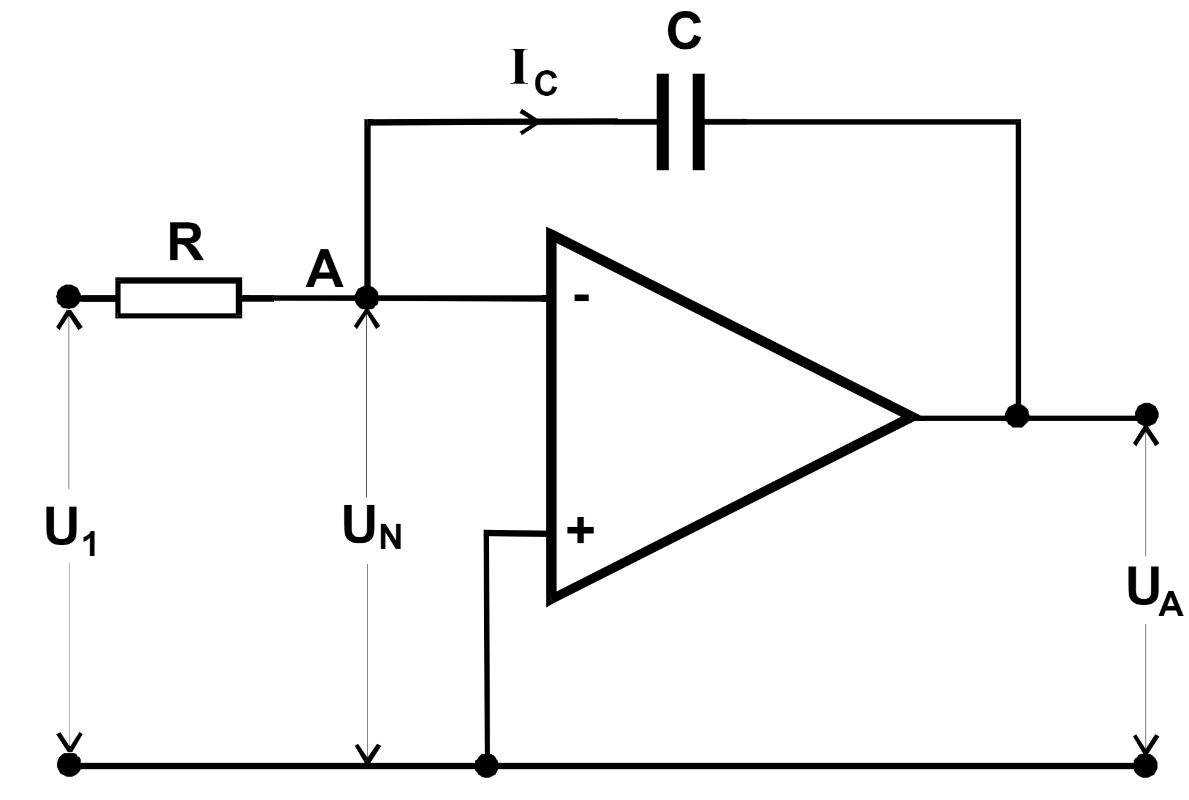
\includegraphics[width=1.0\linewidth]{integrator.PNG}
        \caption{Schaltbild eines Umkehr-Integrators \cite{V51}.}
        \label{fig:integrator-integrator}
    \end{subfigure}
    \begin{subfigure}{.49\linewidth}
        \centering
        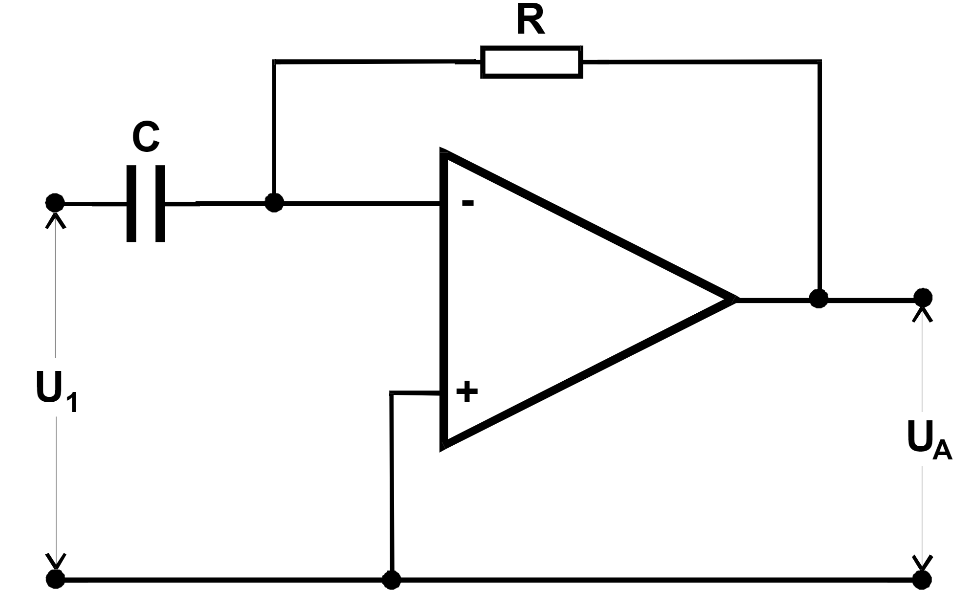
\includegraphics[width=1.0\linewidth]{differentiator.PNG}
        \caption{Schaltbild eines Umkehr-Differentiators \cite{V51}.}
        \label{fig:integrator-differentiator}
    \end{subfigure}
    \caption{Linearverstärker mit Kondensator.}
    \label{fig:integrator}
\end{figure}


\subsection{Schmitt-Trigger}
\label{subsec:schmitt_trigger}
Der Operationsverstärker kann als Schalter genutzt werden. Statt, wie bisher
einen Teil der Ausgangsspannung auf invertierenden Eingang zu geben (Gegenkopplung),
wird dieser Anteil auf den nicht-invertierenden Eingang gegeben (Mitkopplung).
Damit wird das eigene Ausgangssignal verstärkt und der Operationsverstärker erreicht
schnell die Sättigungsspannung $U_\text{B}$.
\begin{align}
    U_\text{A} =
    \begin{cases}
        +U_\text{B} &: U_1 > \frac{R_1}{R_\text{P}}U_\text{B} \\
        -U_\text{B} &: U_1 < -\frac{R_1}{R_\text{P}}U_\text{B}\,,
    \end{cases}
    \label{eqn:schmitt}
\end{align}
mit der Betriebsspannung $U_\text{B}$. Der Schmitt-Trigger besitzt also im Gegensatz
zu anderen Schaltern nicht nur eine Schaltschwelle, sondern zwei. Mit dieser Eigenschaft eignet sich der Schmitt-Trigger
besonders gut zur bereinigung von digitalen Signalen.
Die entsprechende Schaltung ist in Abbildung \ref{fig:schmitt_trigger}
dargestellt.
\begin{figure}[H]
    \centering
    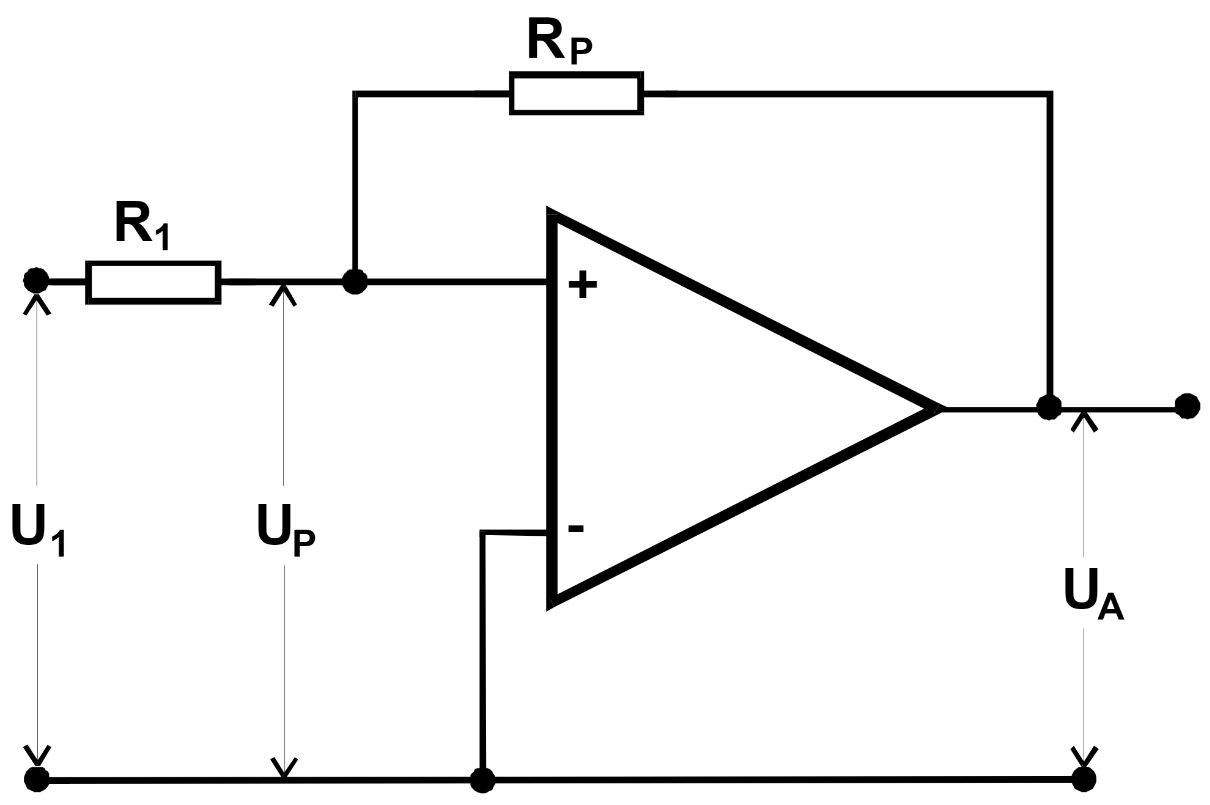
\includegraphics[width=0.5\linewidth]{schmitt_trigger.PNG}
    \caption{
        Schaltbild eines Operationsverstärkers, der als Schmitt-Trigger
        genutzt wird.
    }
    \label{fig:schmitt_trigger}
\end{figure}
\clearpage
\subsection{Signalgenerator}
\label{subsec:signalgenerator}
Schließlich können mit Hilfe eines Operationsverstärkers verschiedene
Signalspannungen erzeugt werden. Dazu wird jeweils eine Mehrzahl von OPVs
miteinander verschaltet.


\subsubsection{Erzeugung von Sinusschwingungen}
\label{subsubsec:sinusschwingungen}
Durch Kombination zweier Integratoren mit einem Umkehrverstärker lassen sich
gedämpfte Sinusschwingungen erzeugen.
Die Schaltung kann durch eine Differentialgleichung 2. Ordung beschrieben
werden und liefert die Lösung
\begin{equation}
    U_\text{A}(t) = U_0 \exp\!\left( \frac{\eta t}{\num{20} RC} \right)
                        \sin\!\left( \frac{t}{RC} \right)\,.
    \label{eqn:oszi}
\end{equation}
Dabei ist $\num{-1} < \eta < \num{1}$ durch das Potentiometer $P$ einzustellen.
Die Schwingungsdauer beträgt dabei $T = 2\pi RC$, die Abklingzeit
$\tau = 20 RC / |\eta|$. Damit sollte die Amplitude für $\eta = \num{0}$
konstant bleiben.
Das Schaltbild zu einem Sinusgenerator ist in Abbildung \ref{fig:sinus}
dargestellt.
\begin{figure}[H]
    \centering
    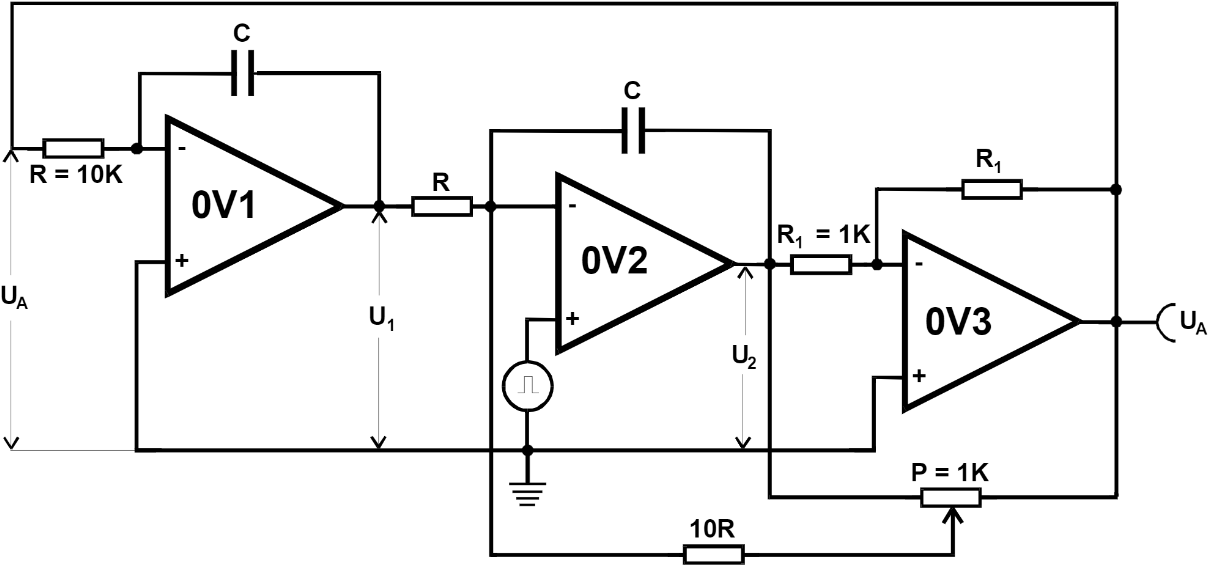
\includegraphics[width=0.9\linewidth]{sinus.PNG}
    \caption{
        Schaltbild eines Sinusgenerators. Es werden zwei Integrationsglieder
        und ein Umkehrverstärker verbaut \cite{V51}.
    }
    \label{fig:sinus}
\end{figure}

\section{Durchführung}
\label{sec:durchführung}
%[16:36, 9.7.2018] tim s: ADEFH


Mit Hilfe der Schaltung \ref{fig:linear} wird zunächst der Frequenzgang eines
gegengekoppelten Verstärkers bei vier verschiedenen Verstärkungsgraden $V'$
und über mehrere Zehnerpotenzen untersucht. \\
\\
\noindent
Als nächstes wird ein Umkehr-Integrator, wie in Abbildung
\ref{fig:integrator-integrator} zur Überprüfung der Beziehung
$U_a \approx \frac{1}{\nu}$ aufgebaut. Außerdem werden
verschiedene Signalformen eines Funktionsgenerators auf den Integrator gegeben und
die Ausgangssignale an einem Oszilloskop beobachtet. \\
\\
\noindent
Daraufhin wird ein Umkehr-Differentiator nach der Schaltung in Abbildung
\ref{fig:integrator-differentiator} verwendet und wie beim Umkehr-Integrator
verfahren. \\
\\
\noindent
Danach wird ein Schmitt-Trigger wie in Abbildung \ref{fig:schmitt_trigger} aufgebaut.
Auf den Eingang wird ein Sinus-Signal gegeben. Das Ausgangssignal wird erneut an einem
Oszilloskop beobachtet und die Spannungsschwelle vermessen. \\
\\
\noindent
Als Letztes werden gedämpfte Schwingungen untersucht. Zur Realisierung einer gedämpften
Schwingung wird die Schaltung nach Abbildung \ref{fig:sinus} verwendet. Zur Erzeugung
der Schwingung wird vor dem OPV 2 ein Rechteckgenerator mit eingebaut. An einem
Potentiometer wird dann $\eta = -1$ für eine gedämpfte Schwingung eingestellt.
\clearpage
\section{Auswertung}
\label{sec:auswertung}
\subsection{Fehlerrechnung}
Für die Fehlerrechnung sowie den mathematischen Teil der Auswertung wird auf
$\textsc{Python}$ zurückgegriffen:\\
Regressionen sowie deren Fehler wurden durch die $\textsc{Scipy}$ \cite{scipy} Funktion
$\textsc{curve-fit}$ durchgeführt. Grafiken wurden mit $\textsc{Matplotlib}$ \cite{matplotlib}
erstellt.
Fehlerfortpflanzung wird durch die Bibliothek
$\textsc{Uncertainties}$ \cite{uncertainties} automatisiert.

\subsection{Gegengekoppelter Linearverstärker}
Bei dem gegengekoppelter Linearverstärker werden die Werte aus Tabelle \ref{tab:messwerte1}
gemessen. Die Graphen dazu sind in den Abbildungen \ref{fig:plot} bis \ref{fig:plot4}
zu sehen. Als Eingangsspannung dienten dabei die Spannungen in Tabelle \ref{tab:eingangs}.
\begin{table}[H]
  \centering
  \caption{Die Eingangsspannungen, Widerstandsverhältnisse, Verstärkungsfaktoren, und $\log{\frac{V^\prime}{\sqrt{2}}}$.}
  \label{tab:eingangs}
  \begin{tabular}{c c c c c}
    \toprule
    Schaltung & $U_\text{e}$ & $\frac{R_\text{N}}{R_1}$ & $V^\prime$ & $\log{\frac{V^\prime}{\sqrt{2}}}$ \\
    \midrule
    1 & $\SI{260}{\milli\volt}$   & $\SI{469}{\ohm}/\SI{468}{\ohm} \approx 1$        & $\SI{0.998}{}$ & $\SI{-0.348}{}$ \\
    2 & $\SI{258}{\milli\volt}$   & $\SI{996}{\ohm}/\SI{468}{\ohm} \approx 2$        & $\SI{0.990}{}$ & $\SI{-0.356}{}$ \\
    3 & $\SI{257.5}{\milli\volt}$ & $\SI{10}{\kilo\ohm}/\SI{468}{\ohm} \approx 21$   & $\SI{0.992}{}$ & $\SI{-0.354}{}$ \\
    4 & $\SI{257.5}{\milli\volt}$ & $\SI{33.1}{\kilo\ohm}/\SI{468}{\ohm} \approx 71$ & $\SI{0.951}{}$ & $\SI{-0.396}{}$ \\
    \bottomrule
  \end{tabular}
\end{table}
\noindent
Die Messwerte werden durch die jeweilige Eingangsspannung geteilt, um auf den effektiven
Verstärkungsfaktor $V^\prime_\text{eff}$ zu kommen. Der jeweils erste Wert stellt den
Verstärkungsfaktor $V^\prime$ dar und der entsprechende Wert
steht zusammen mit dem Wert $\log{\frac{V^\prime}{\sqrt{2}}}$ und dem Widerstandsverhältnis
in Tabelle \ref{tab:eingangs}. Die Frequenzen und die effektiven
Verstärkungsfaktoren werden logarithmiert und stehen in Tabelle \ref{tab:logwerte}.
$\log{\frac{V^\prime}{\sqrt{2}}}$ wird als Konstante in die Plots eingezeichnet. Die
Bandbreite ist bis zu dem Schnittpunkt der beiden Kurven definiert. Also wird
eine Gerade, der Form:
\begin{equation*}
  \log{V^\prime_\text{eff}} (\log{\nu}) = m \cdot \log{\nu} + b,
\end{equation*}
durch die fallende Flanke der Messwerte gefittet und die Parameter in der entsprechenden
Umkehrfunktion
\begin{equation*}
  \log{\nu} (\log{V^\prime_\text{eff}}) = \frac{\log{V^\prime_\text{eff}}-b}{m}
\end{equation*}
verwendet um durch Einsetzen von $\log{\frac{V^\prime}{\sqrt{2}}}$ den Wert für $\log{\nu^\prime_g}$
zu berechnen. Durch exponentieren folgt die Grenzfrequenz $\nu^\prime_g$.
Für den Fit werden bei Schaltung 1 die letzten sechs Werte verwendet.
Bei Schaltung 2 sind es die letzten acht. Bei Schaltung 3 alle außer die ersten sechs
und bei Schaltung 4 alle außer die ersten zwei und die letzten vier.
Als Parameter ergeben sich für die vier Schaltungen die Werte in Tabelle \ref{tab:parameter}.
In selbiger stehen auch die Grenzfrequenzen und das Verstärkungs-Bandbreite-Produkt
$\nu^\prime_g \cdot V^\prime$.
\begin{table}[H]
  \centering
  \caption{Die Parameter der Fits, Grenzfrequenzen und Verstärkung-Bandbreite-Produkte der Schaltungen.}
  \label{tab:parameter}
  \begin{tabular}{c c c c c}
    \toprule
    Schaltung & m & b & $\nu^\prime_g$ in $\si{\kilo\hertz}$ & $\nu^\prime_g \cdot V^\prime$ in $\si{\kilo\hertz}$ \\
    \midrule
    1 & $\SI{-0.550(15)}{}$ & $\SI{3.51(11)}{}$ & $\SI{1.12(32)e3}{}$ & $\SI{1.12(32)e3}{}$ \\
    2 & $\SI{-0.516(14)}{}$ & $\SI{3.06(9)}{}$  & $\SI{7.6(19)e2}{}$ & $\SI{7.5(19)e2}{}$ \\
    3 & $\SI{-0.704(14)}{}$ & $\SI{2.98(7)}{}$ & $\SI{115(16)}{}$ & $\SI{114(16)}{}$ \\
    4 & $\SI{-0.760(11)}{}$ & $\SI{2.39(6)}{}$ & $\SI{38.9(35)}{}$ & $\SI{37.0(34)}{}$ \\
    \bottomrule
  \end{tabular}
\end{table}

\noindent
Als stark vereinfachtes Ersatzschaltbild eignet sich hierbei ein $RC$-Tiefpass.
Da die Eingangswiderstände des Operationsverstärkers sehr groß sind und einige
der Bauteile im inneren des Verstärkers (z.B. Dioden und Transistoren) eine
wenn auch kleine Sperrschichtkapazität besitzen zeigt sich bei entsprechend hohen Frequenzen
ein kapazitives Verhalten.\\

\noindent
Zur Abschätzung von $V$ wird die Formel
\begin{equation}
  \frac{1}{V^\prime} \approx \frac{1}{V}+\frac{R_1}{R_\text{N}}
\end{equation}
aus der Anleitung verwendet. Dazu wird diese auf $V$ umgeformt und für die einzelnen Schaltungen
$V^\prime$ sowie die Widerstände eingesetzt.
Die Ergebnisse stehen in Tabelle \ref{tab:vabsch}.
\begin{table}[H]
  \centering
  \caption{Die Ergebnisse der Abschätzung von $V$.}
  \label{tab:vabsch}
  \begin{tabular}{c c}
    \toprule
    Schaltung & $V$\\
    \midrule
    1 & $\approx 246$ \\
    2 & $\approx 2  $ \\
    3 & $\approx 1  $ \\
    4 & $\approx 1  $ \\
    \bottomrule
  \end{tabular}
\end{table}
\begin{table}
  \centering
  \caption{Die gemessenen Spannungen für den gegengekoppelten Linearverstärker.}
  \label{tab:messwerte1}
  \begin{tabular}{c c c c c c c c}
    \toprule
    \multicolumn{2}{c}{Schaltung: 1} & \multicolumn{2}{c}{2} & \multicolumn{2}{c}{3} & \multicolumn{2}{c}{4} \\
    $\nu$ in $\si{\kilo\hertz}$ & $U_\text{A}$ in $\si{\milli\volt}$ & $\nu$ in $\si{\kilo\hertz}$ & $U_\text{A}$ in $\si{\milli\volt}$ & $\nu$ in $\si{\kilo\hertz}$ & $U_\text{A}$ in $\si{\milli\volt}$ & $\nu$ in $\si{\kilo\hertz}$ & $U_\text{A}$ in $\si{\milli\volt}$ \\
    \midrule
    0,4   & 259,5 & 0,4  & 255,5 & 0,4  & 255,5 & 0,4  & 245   \\
    16,4  & 259,5 & 20   & 255,5 & 16,4 & 251,5 & 16,4 & 225   \\
    32,4  & 259,5 & 40   & 255,5 & 32,4 & 239   & 32,4 & 183   \\
    48,35 & 259,5 & 80   & 254,5 & 48,4 & 230   & 48,4 & 148,5 \\
    64,35 & 259,5 & 120  & 248   & 66,4 & 213   & 64   & 120,5 \\
    80,3  & 259,5 & 160  & 251   & 82,4 & 203   & 80   & 103,5 \\
    96,3  & 259,5 & 200  & 243   & 96,4 & 191   & 96   & 88,5  \\
    112   & 259,5 & 240  & 239   & 112  & 181   & 112  & 78,5  \\
    128   & 258   & 280  & 234   & 128  & 167   & 128  & 72,5  \\
    144   & 256,5 & 320  & 234   & 144  & 155   & 144  & 64,5  \\
    160   & 256,5 & 360  & 223   & 160  & 146,5 & 160  & 60,5  \\
    176   & 256,5 & 400  & 221   & 176  & 136,5 & 176  & 55,5  \\
    192   & 256,5 & 500  & 211   & 192  & 128,5 & 192  & 53,5  \\
    208   & 256,5 & 550  & 207   & 208  & 121,5 & 208  & 48    \\
    224   & 255   & 600  & 200   & 224  & 116,5 & 224  & 45    \\
    240   & 255   & 650  & 195   & 240  & 109,5 & 240  & 44    \\
    256   & 255   & 700  & 187   & 256  & 104,5 & 256  & 40    \\
    272   & 252   & 750  & 183   & 272  & 99,5  & 272  & 39    \\
    288   & 252   & 800  & 177   & 288  & 94,5  & 288  & 39    \\
    304   & 250,5 & 850  & 170   & 304  & 90,5  & 304  & 36    \\
    320   & 250,5 & 900  & 165   & 320  & 88,5  & 320  & 34    \\
    336   & 249   & 950  & 161   & 336  & 84,5  & 336  & 32    \\
    352   & 249   & 1000 & 156   & 352  & 80,5  & 352  & 32    \\
    368   & 244,5 &      &       & 368  & 76,5  & 368  & 32    \\
    384   & 244,5 &      &       & 384  & 76,5  & 384  & 32    \\
    400   & 244,5 &      &       & 400  & 72,5  & 400  & 32    \\
    1181  & 182   &      &       &      &       &      &       \\
    1750  & 143,5 &      &       &      &       &      &       \\
    1930  & 136   &      &       &      &       &      &       \\
    1000  & 195,5 &      &       &      &       &      &       \\
    900   & 204,5 &      &       &      &       &      &       \\
    800   & 211   &      &       &      &       &      &       \\
    2000  & 133   &      &       &      &       &      &       \\
    \bottomrule
  \end{tabular}
\end{table}
\begin{table}
  \centering
  \caption{Die logerithmierten Werte von Frequenz und effektivem Verstärkungsfaktor.}
  \label{tab:logwerte}
  \begin{tabular}{c c c c c c c c}
    \toprule
    \multicolumn{2}{c}{Schaltung: 1} & \multicolumn{2}{c}{2} & \multicolumn{2}{c}{3} & \multicolumn{2}{c}{4} \\
    $\log{\nu}$ & $\log{V^\prime_\text{eff}}$ & $\log{\nu}$ & $\log{V^\prime_\text{eff}}$ & $\log{\nu}$ & $\log{V^\prime_\text{eff}}$ & $\log{\nu}$ & $\log{V^\prime_\text{eff}}$ \\
    \midrule
    $\SI{-0.916}{}$ & $\SI{-0.00192}{}$ & $\SI{-0.916}{}$ & $\SI{-0.00974}{}$ & $\SI{-0.916}{}$ & $\SI{-0.00780}{}$ & $\SI{-0.916}{}$ & $\SI{-0.0498}{}$ \\
    $\SI{ 2.80}{}$  & $\SI{-0.00192}{}$ & $\SI{ 3.00}{}$ & $\SI{-0.00974}{}$ & $\SI{ 2.80}{}$  & $\SI{-0.0236}{}$ & $\SI{ 2.80}{}$ & $\SI{-0.135}{}$  \\
    $\SI{ 3.48}{}$  & $\SI{-0.00192}{}$ & $\SI{ 3.69}{}$ & $\SI{-0.00974}{}$ & $\SI{ 3.48}{}$  & $\SI{-0.0746}{}$ & $\SI{ 3.48}{}$ & $\SI{-0.342}{}$  \\
    $\SI{ 3.88}{}$  & $\SI{-0.00192}{}$ & $\SI{ 4.38}{}$ & $\SI{-0.0137}{}$  & $\SI{ 3.88}{}$  & $\SI{-0.113}{}$ & $\SI{ 3.88}{}$ & $\SI{-0.550}{}$  \\
    $\SI{ 4.16}{}$  & $\SI{-0.00192}{}$ & $\SI{ 4.79}{}$ & $\SI{-0.0395}{}$  & $\SI{ 4.20}{}$  & $\SI{-0.190}{}$ & $\SI{ 4.16}{}$ & $\SI{-0.759}{}$  \\
    $\SI{ 4.39}{}$  & $\SI{-0.00192}{}$ & $\SI{ 5.08}{}$ & $\SI{-0.0275}{}$  & $\SI{ 4.41}{}$  & $\SI{-0.238}{}$ & $\SI{ 4.38}{}$ & $\SI{-0.911}{}$  \\
    $\SI{ 4.57}{}$  & $\SI{-0.00192}{}$ & $\SI{ 5.30}{}$ & $\SI{-0.0599}{}$  & $\SI{ 4.57}{}$  & $\SI{-0.299}{}$ & $\SI{ 4.56}{}$ & $\SI{-1.07}{}$   \\
    $\SI{ 4.72}{}$  & $\SI{-0.00192}{}$ & $\SI{ 5.48}{}$ & $\SI{-0.0765}{}$  & $\SI{ 4.72}{}$  & $\SI{-0.353}{}$ & $\SI{ 4.72}{}$ & $\SI{-1.19}{}$   \\
    $\SI{ 4.85}{}$  & $\SI{-0.00772}{}$ & $\SI{ 5.63}{}$ & $\SI{-0.0976}{}$  & $\SI{ 4.85}{}$  & $\SI{-0.433}{}$ & $\SI{ 4.85}{}$ & $\SI{-1.27}{}$   \\
    $\SI{ 4.97}{}$  & $\SI{-0.0136}{}$  & $\SI{ 5.77}{}$ & $\SI{-0.0976}{}$  & $\SI{ 4.97}{}$  & $\SI{-0.508}{}$ & $\SI{ 4.97}{}$ & $\SI{-1.38}{}$   \\
    $\SI{ 5.08}{}$  & $\SI{-0.0136}{}$  & $\SI{ 5.89}{}$ & $\SI{-0.146}{}$   & $\SI{ 5.08}{}$  & $\SI{-0.564}{}$ & $\SI{ 5.08}{}$ & $\SI{-1.45}{}$   \\
    $\SI{ 5.17}{}$  & $\SI{-0.0136}{}$  & $\SI{ 5.99}{}$ & $\SI{-0.155}{}$   & $\SI{ 5.17}{}$  & $\SI{-0.635}{}$ & $\SI{ 5.17}{}$ & $\SI{-1.53}{}$   \\
    $\SI{ 5.26}{}$  & $\SI{-0.0136}{}$  & $\SI{ 6.21}{}$ & $\SI{-0.201}{}$   & $\SI{ 5.26}{}$  & $\SI{-0.695}{}$ & $\SI{ 5.26}{}$ & $\SI{-1.57}{}$   \\
    $\SI{ 5.34}{}$  & $\SI{-0.0136}{}$  & $\SI{ 6.31}{}$ & $\SI{-0.220}{}$   & $\SI{ 5.34}{}$  & $\SI{-0.751}{}$ & $\SI{ 5.34}{}$ & $\SI{-1.68}{}$   \\
    $\SI{ 5.41}{}$  & $\SI{-0.0194}{}$  & $\SI{ 6.40}{}$ & $\SI{-0.255}{}$   & $\SI{ 5.41}{}$  & $\SI{-0.793}{}$ & $\SI{ 5.41}{}$ & $\SI{-1.74}{}$   \\
    $\SI{ 5.48}{}$  & $\SI{-0.0194}{}$  & $\SI{ 6.48}{}$ & $\SI{-0.280}{}$   & $\SI{ 5.48}{}$  & $\SI{-0.855}{}$ & $\SI{ 5.48}{}$ & $\SI{-1.77}{}$   \\
    $\SI{ 5.55}{}$  & $\SI{-0.0194}{}$  & $\SI{ 6.55}{}$ & $\SI{-0.322}{}$   & $\SI{ 5.55}{}$  & $\SI{-0.902}{}$ & $\SI{ 5.55}{}$ & $\SI{-1.86}{}$   \\
    $\SI{ 5.61}{}$  & $\SI{-0.0313}{}$  & $\SI{ 6.62}{}$ & $\SI{-0.343}{}$   & $\SI{ 5.61}{}$  & $\SI{-0.951}{}$ & $\SI{ 5.61}{}$ & $\SI{-1.89}{}$   \\
    $\SI{ 5.66}{}$  & $\SI{-0.0313}{}$  & $\SI{ 6.68}{}$ & $\SI{-0.377}{}$   & $\SI{ 5.66}{}$  & $\SI{-1.00}{}$  & $\SI{ 5.66}{}$ & $\SI{-1.89}{}$   \\
    $\SI{ 5.72}{}$  & $\SI{-0.0372}{}$  & $\SI{ 6.75}{}$ & $\SI{-0.417}{}$   & $\SI{ 5.72}{}$  & $\SI{-1.05}{}$  & $\SI{ 5.72}{}$ & $\SI{-1.97}{}$   \\
    $\SI{ 5.77}{}$  & $\SI{-0.0372}{}$  & $\SI{ 6.80}{}$ & $\SI{-0.447}{}$   & $\SI{ 5.77}{}$  & $\SI{-1.07}{}$  & $\SI{ 5.77}{}$ & $\SI{-2.02}{}$   \\
    $\SI{ 5.82}{}$  & $\SI{-0.0432}{}$  & $\SI{ 6.86}{}$ & $\SI{-0.472}{}$   & $\SI{ 5.82}{}$  & $\SI{-1.11}{}$  & $\SI{ 5.82}{}$ & $\SI{-2.09}{}$   \\
    $\SI{ 5.86}{}$  & $\SI{-0.0432}{}$  & $\SI{ 6.91}{}$ & $\SI{-0.503}{}$   & $\SI{ 5.86}{}$  & $\SI{-1.16}{}$  & $\SI{ 5.86}{}$ & $\SI{-2.09}{}$   \\
    $\SI{ 5.91}{}$  & $\SI{-0.0615}{}$  &                &                   & $\SI{ 5.91}{}$  & $\SI{-1.21}{}$  & $\SI{ 5.91}{}$ & $\SI{-2.09}{}$   \\
    $\SI{ 5.95}{}$  & $\SI{-0.0615}{}$  &                &                   & $\SI{ 5.95}{}$  & $\SI{-1.21}{}$  & $\SI{ 5.95}{}$ & $\SI{-2.09}{}$   \\
    $\SI{ 5.99}{}$  & $\SI{-0.0615}{}$  &                &                   & $\SI{ 5.99}{}$  & $\SI{-1.27}{}$  & $\SI{ 5.99}{}$ & $\SI{-2.09}{}$   \\
    $\SI{ 6.68}{}$  & $\SI{-0.209}{}$   &                &                   &                 &                 &                &                  \\
    $\SI{ 6.80}{}$  & $\SI{-0.240}{}$   &                &                   &                 &                 &                &                  \\
    $\SI{ 6.91}{}$  & $\SI{-0.285}{}$   &                &                   &                 &                 &                &                  \\
    $\SI{ 7.07}{}$  & $\SI{-0.357}{}$   &                &                   &                 &                 &                &                  \\
    $\SI{ 7.47}{}$  & $\SI{-0.594}{}$   &                &                   &                 &                 &                &                  \\
    $\SI{ 7.57}{}$  & $\SI{-0.648}{}$   &                &                   &                 &                 &                &                  \\
    $\SI{ 7.60}{}$  & $\SI{-0.670}{}$   &                &                   &                 &                 &                &                  \\
    \bottomrule
  \end{tabular}
\end{table}
\begin{figure}
  \centering
  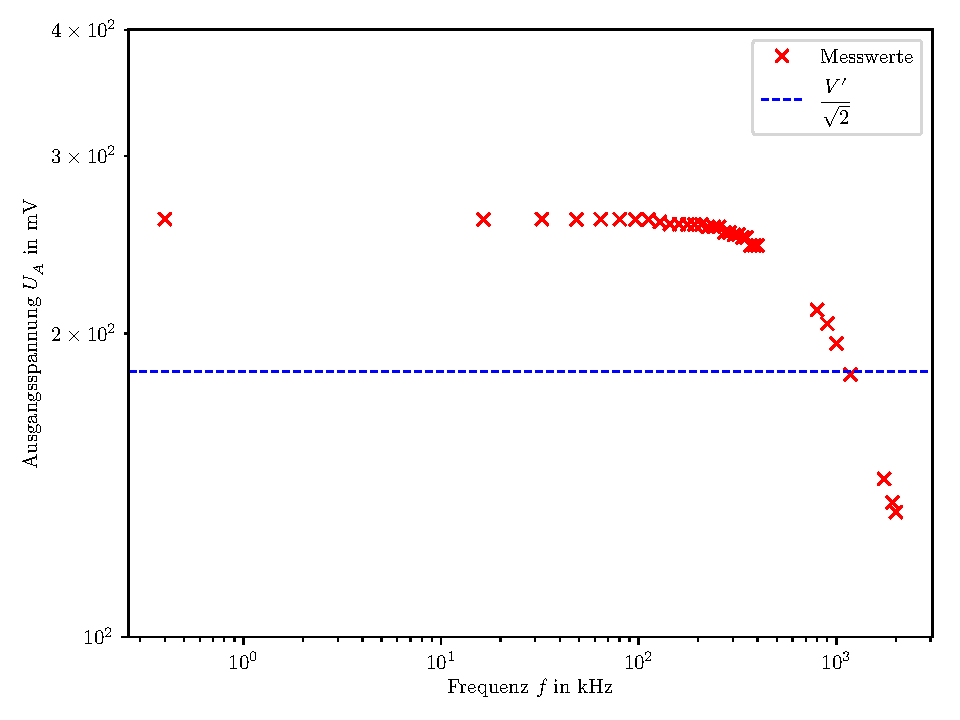
\includegraphics[width=0.8\textwidth]{plot.pdf}
  \caption{Messwerte mit Schaltung 1.}
  \label{fig:plot}
\end{figure}
\begin{figure}
  \centering
  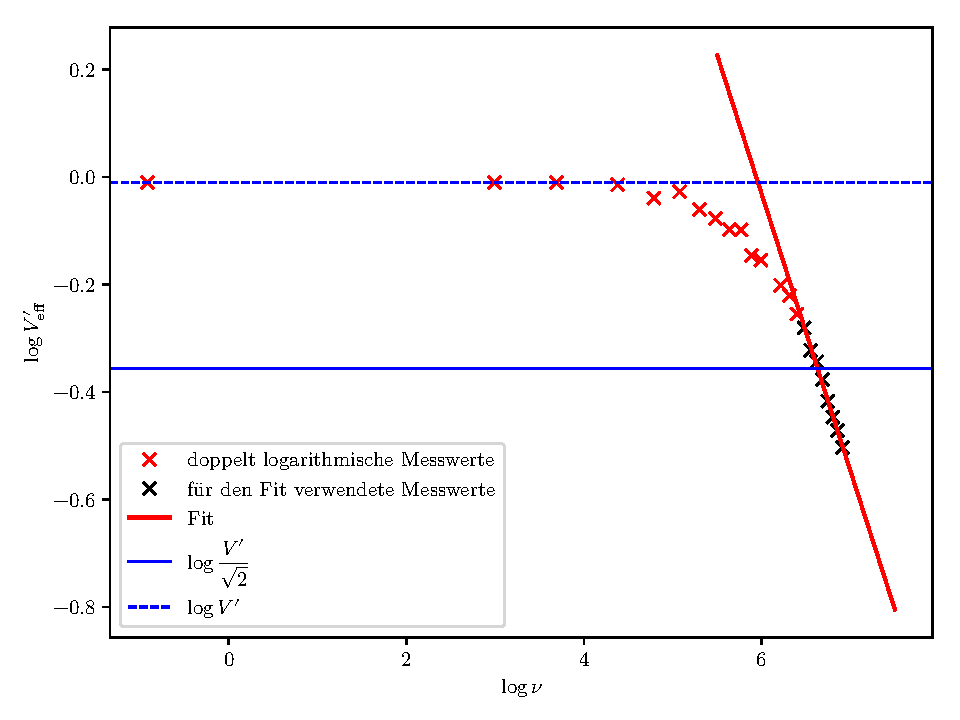
\includegraphics[width=0.8\textwidth]{plot2.pdf}
  \caption{Messwerte mit Schaltung 2.}
  \label{fig:plot2}
\end{figure}
\begin{figure}
  \centering
  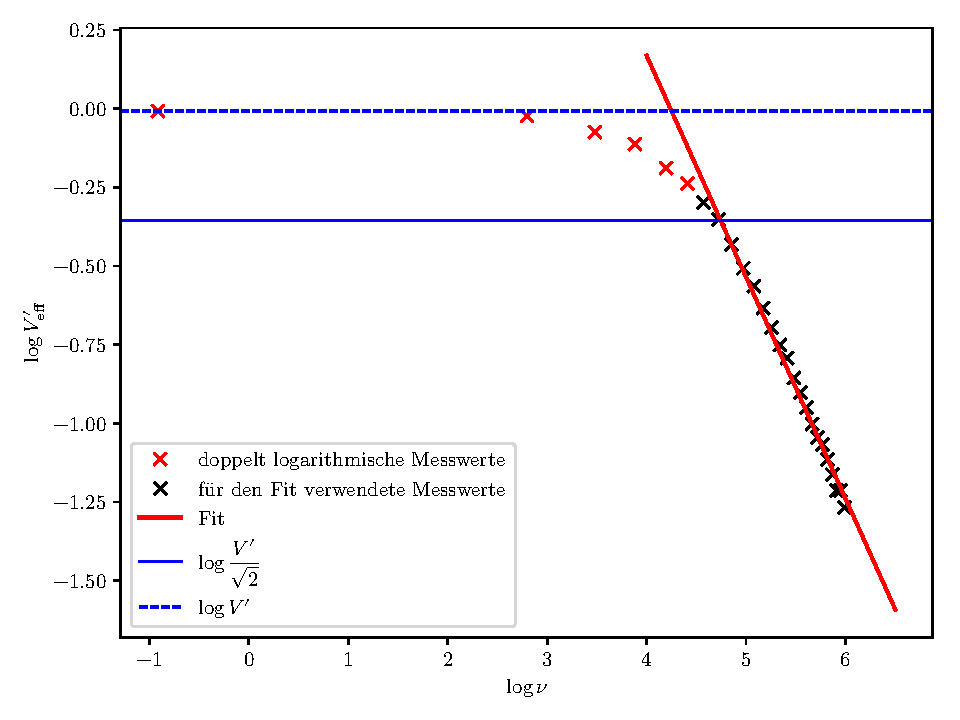
\includegraphics[width=0.8\textwidth]{plot3.pdf}
  \caption{Messwerte mit Schaltung 3.}
  \label{fig:plot3}
\end{figure}
\begin{figure}[H]
  \centering
  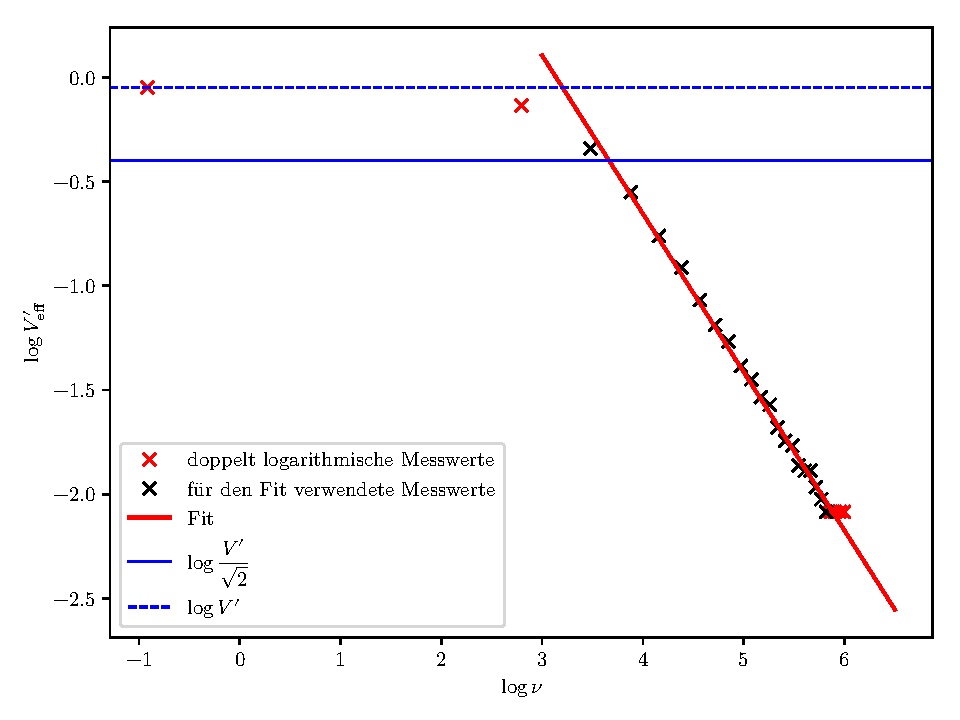
\includegraphics[width=0.8\textwidth]{plot4.pdf}
  \caption{Messwerte mit Schaltung 4.}
  \label{fig:plot4}
\end{figure}

\subsection{Differentiator und Integrator}
Diese beiden Schaltungen haben aufgrund eines technischen Defektes nicht funktioniert.
In dem Signal waren ungewollte höher frequente Schwingungen zu sehen.
Dadurch war eine Aufnahme des Frequenzverhaltens unmöglich. Das Problem ließ sich
auch nicht beheben. Am Ende hat sich herrausgestellt, dass es scheinbar ein defekter Anschluss
am Entwicklerboard war.

\subsection{Schmitt-Trigger}
In Abbildung \ref{fig:schmitttrigg} ist eine Bildschirmaufnahme des Eingangs- und
des Ausgangssignals des Schmitt-Triggers zu sehen. Dabei ist das Sinus-Signal das Eingangssignal
und das Rechteck-Signal das Ausgangssignal.
\begin{figure}[H]
  \centering
  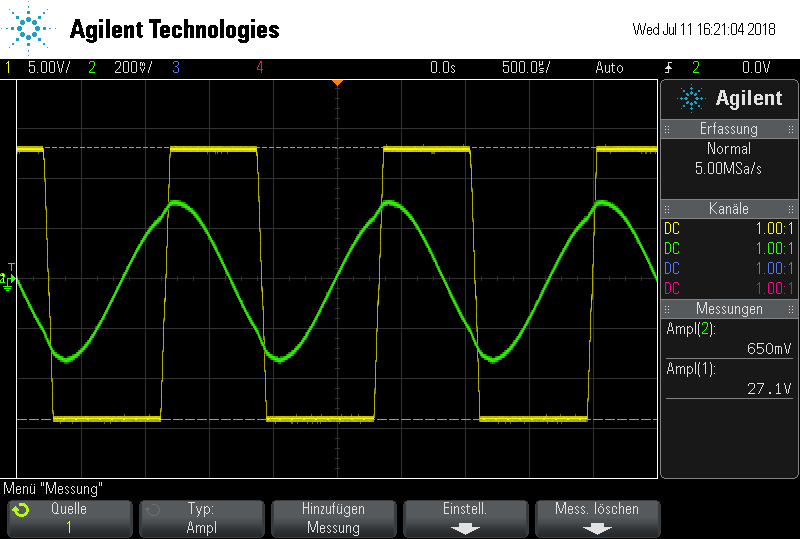
\includegraphics[width=0.8\textwidth]{schmitt.png}
  \caption{Bildschirmaufnahme Schmitt-Trigger.}
  \label{fig:schmitttrigg}
\end{figure}
\noindent
Die gemessenen Scheitelspannungen sind:
\begin{align*}
  U_\text{e,ein} &= \SI{278(5)}{\milli\volt} \\
  U_\text{e,aus} &= \SI{-249(5)}{\milli\volt}.
\end{align*}
Als Ausgangsspannung werden
\begin{align*}
  U_\text{B} &= \SI{13.0(1)}{\volt} \\
  -U_\text{B} &= \SI{-14.0(1)}{\volt}
\end{align*}
gemessen und die verwendeten Widerstände betragen:
\begin{align*}
  R_1 &= \SI{470(4)}{\ohm} \\
  R_\text{P} &= \SI{33.1(2)}{\kilo\ohm}.
\end{align*}
Mit diesen Werten ergeben sich nach den Formeln \eqref{eqn:schmitt} theoretische
Werte für die Scheitelspannungen:
\begin{align*}
  U_\text{e,ein} &= \SI{199(3)}{\milli\volt} \\
  U_\text{e,aus} &= \SI{-185(2)}{\milli\volt}.
\end{align*}

\subsection{Oszillator Schaltung}
Für diese Schaltung war aus dem gleichen Grund, wie bei den Differentiator- und
Integratorschaltungen, keine Messung möglich. Die Werte haben wir daher
von dem Betreuer erhalten. Sie sind in Abbildung \ref{fig:plot5} dargestellt.
\begin{figure}[H]
  \centering
  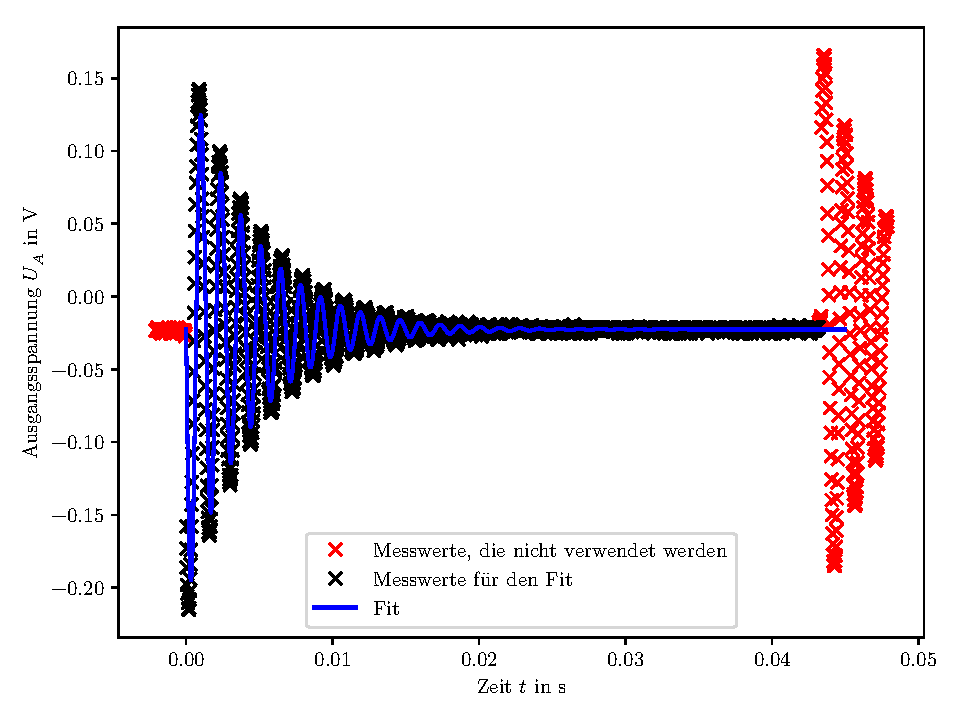
\includegraphics[width=0.8\textwidth]{plot5.pdf}
  \caption{Werte und Fit zu der Oszillator Schaltung.}
  \label{fig:plot5}
\end{figure}
\noindent
Es werden alle Werte aussortiert, die vor der ersten Anregung und nach der zweiten
Anregung durch die Rechteckspannung liegen. Die restlichen Werte werden anschließend
nach einer Funktion
\begin{equation*}
  f(t) = a \cdot \exp{\left(\frac{-1 \cdot (t-b)}{20 \cdot c}\right)} \cdot \sin{\left(\frac{(t-b)}{c}\right)} + d
\end{equation*}
gefittet.
Als Startwerte für den Fit dienen dabei:
\begin{align*}
  a &= \SI{200}{\milli\volt} \\
  b &= \SI{0}{\second} \\
  c &= \SI{224}{\micro\second} \\
  d &= \SI{-20}{\milli\volt}.
\end{align*}
Bei dem Fit ergeben sich folgende Parameter:
\begin{align*}
  a &= \SI{-210.5(2)}{\milli\volt} \\
  b &= \SI{168.9(3)}{\micro\second} \\
  c &= \SI{225.00(2)}{\micro\second} \\
  d &= \SI{-22.74(3)}{\milli\volt}.
\end{align*}
Die verwendeten Bauteile haben die Werte:
\begin{align*}
  R &= \SI{9.96}{\kilo\ohm} \\
  C_1 &= \SI{21.5}{\nano\farad} \\
  C_2 &= \SI{23.6}{\nano\farad} \\
  10R &= \SI{99.6}{\kilo\ohm} \\
  R_1 &= \SI{996}{\ohm}
\end{align*}
Da die Werte der Kapazitäten eine etwas größere Differenz besitzen, werden diese
beiden Werte gemittelt. Der Mittelwert ist: $C = \SI{22.6(10)}{\nano\farad}$.
Damit wird jetzt der Theoriewert für die Konstante $c$ des Fits berechnet.
Nach Formel \eqref{eqn:oszi} folgt:
\begin{equation*}
  R \cdot C = \SI{225(10)}{\micro\second}
\end{equation*}
und
\begin{equation*}
  \tau = 20\cdot R C = \SI{4.49(21)}{\milli\second}.
\end{equation*}
Aus dem Fit ergibt sich
\begin{equation*}
  \tau = 20 \cdot c = \SI{4.4999(4)}{\milli\second}.
\end{equation*}
\clearpage
\section{Diskussion}
\label{diskussion}
\begin{table}[H]
  \centering
  \caption{Die Ergebnisse zu dem gegengekoppelten Linearverstärker.}
  \label{tab:ergebnisse}
  \begin{tabular}{c c c c c c}
    \toprule
    Schaltung & $V^\prime$ & $\frac{R_\text{N}}{R_1}$ & $\nu^\prime_g$ in $\si{\kilo\hertz}$ & $\nu^\prime_g \cdot V^\prime$ in $\si{\kilo\hertz}$ & $V$ \\
    \midrule
    1 & $\SI{0.998}{}$ & $\approx 1$  & $\SI{1.12(32)e3}{}$ & $\SI{1.12(32)e3}{}$ & $\approx 246$ \\
    2 & $\SI{0.990}{}$ & $\approx 2$  & $\SI{7.6(19)e2}{}$  & $\SI{7.5(19)e2}{}$  & $\approx 2$   \\
    3 & $\SI{0.992}{}$ & $\approx 21$ & $\SI{115(16)}{}$    & $\SI{114(16)}{}$    & $\approx 1$   \\
    4 & $\SI{0.951}{}$ & $\approx 71$ & $\SI{38.9(35)}{}$   & $\SI{37.0(34)}{}$   & $\approx 1$   \\
    \bottomrule
  \end{tabular}
\end{table}
Auffällig ist, dass bei den gegengekoppelten Linearverstärkerschaltungen die
maximale Ausgangsspannung immer gleich war und etwa der Eingangsspannung entsprach.
Der Verstärkungsfaktor $V^\prime$ ist also immer $\approx 1$. Bei der ersten Schaltung
stimmt das. Doch bei den Anderen müsste er entsprechend dem Widerstandsverhältnis 2, 21 bzw. 71 mal so groß sein.

\noindent
Die Abweichung in $V^\prime$ wirkt sich auf alle damit zusammenhängenden Ergebnisse aus.
Das Verstärkung-Bandbreite-Produkt ist nicht konstant.
Die Ergebnisse der vier Schaltungen diesbezüglich liegen alle in unterschiedlichen Größenordnungen.
Das kann aber nicht vollständig auf die Abweichung in $V^\prime$ zurückgeführt
werden. Selbst mit den Widerstandverhältnissen sind sie nicht konstant.
Also muss es bei den Grenzfrequenzen auch eine Abweichung geben, die allerdings auch
indirekt durch den Verstärkungsfaktor zustande kommen könnte.
Bei der Abschätzung von $V$ ist höchstens der Wert von Schaltung 1 sinnvoll.
Der Wert für Schaltung zwei entspricht ungefähr dem Widerstandsverhältnis und
die Werte für die anderen Schaltungen sind sogar kleiner als das jeweilige
Widerstandsverhältnis. Damit sind sie viel zu klein.
Trotz alledem ist das Tiefpassverhalten des gegengekoppelten Linearverstärkers
gut erkennbar und die Grenzfrequenz nimmt sogar mit zunehmendem Widerstandsverhältnis
ab.

\noindent
Das Problem mit der Ausgangsspannung ließ sich am Ende dadurch lösen,
dass man den Widerstand, welcher zu dem OPV parallel geschaltet wird, "direkt"
in die Schaltung auf dem Entwicklerboard einbaut und nicht "indirekt"
über Verkabelungen anschließt. Dadurch hat die Schmitt-Trigger Schaltung später
gut Funktioniert. Allerdings war die Zeit zu knapp um die ersten Messreihen zu
wiederholen. Die Differentiator- und Integratorschaltungen haben leider aus genannten
Gründen nicht funktioniert.

\noindent
Die Ergebnisse für die Scheitelspannungen des Schmitt-Triggers sind:
\begin{align*}
  \text{Theorie:} U_\text{e,ein} &= \SI{199(3)}{\milli\volt} \\
  \text{Gemessen:} U_\text{e,ein} &= \SI{278(5)}{\milli\volt} \\
  \text{Theorie:} U_\text{e,aus} &= \SI{-185(2)}{\milli\volt} \\
  \text{Gemessen:} U_\text{e,aus} &= \SI{-249(5)}{\milli\volt}
\end{align*}
Der Schmitt-Trigger hat gut funktioniert und seine Aufgabe erfüllt.
Allerdings sind die gemessenen Scheitelspannungen 1,4 mal
so groß, wie die theoretischen Werte.
Eventuell sind dafür die unter der idealen Annahme vernachlässigten Eigenschaften
eines realen OPVs verantwortlich oder es hing ebenfalls mit dem defekten Entwicklerboard
zusammen.

\noindent
Die Ergebnisse für $RC$ bzw. $\tau$ bei der Oszillatorschaltung sind:
\begin{align*}
  &\text{Theorie:}& R \cdot C &= \SI{225(10)}{\micro\second} \\
  &\text{Fit:}& c = R \cdot C &= \SI{225.00(2)}{\micro\second} \\
  &\text{Theorie:}& \tau &= \SI{4.49(21)}{\milli\second} \\
  &\text{Fit:}& \tau &= \SI{4.4999(4)}{\milli\second}.
\end{align*}
Damit entsprechen die Werte aus dem Fit genau den theoretischen Werten.
Die Daten sind demzufolge sehr gut.

\newpage
\nocite{*}
\printbibliography

\end{document}
